\section{Desenho e Implementa��o de RSSF Seguras }\label{sect:sec_secure_wsn_design}
Com o aparecimento das redes sem fios surge tamb�m um novo desafio relacionado com as quest�es de
seguran�a dos dados que circulam na rede, tendo em conta  o meio de comunica��o que � aberto 
e de f�cil acesso. No entanto, a emerg�ncia das RSSF ainda levanta maiores desafios
relacionados com esta problem�tica. Considerando que as RSSF s�o um sub-conjunto das redes
\textit{ad-hoc} (ANET). Veja-se portanto algumas diferen�as entre estas duas
tipologias\cite{VER}:  i) O n�mero de n�s nas RSSF pode ser muito maior que os existentes
numa ANET; ii) Os n�s sensores s�o distr�buidos de forma densa (pr�ximos uns dos outros); iii) Os
sensores s�o mais prop�cios a falhas; iv) A topologia de uma RSSF pode mudar de forma muito mais
frequente; v) Os sensores usam um modo de comunica��o baseado em \textit{broadcast} seguindo um
modelo multi-hop entre pontos, enquanto as ANET s�o orientadas ponto a ponto; vi) Os sensores s�o
limitados em energia, capacidade de armazenamento, mem�ria, processamento e comunica��o.

Tendo estas caracter�sticas em mente, as  diferen�as encontradas correspondem a uma
dificuldade acrescida para manter as propriedades de seguran�a desejadas durante a opera��o de
uma RSSF. Assim, nesta sec��o, importa entender quais as limita��es, qual a arquitectura de
software e de seguran�a, das RSSF,  por forma a que possam resistir a determinados ataques,
que em geral se caracterizam como ataques ao meio de comunica��o e ataques por intrus�o e
captura.
\subsection{Constragimentos � Implementa��o de Seguran�a Impostos pelas RSSF }
A unidade b�sica de uma RSSF � o n� sensor (\textit{mote}). As suas dimens�es reduzidas, resultantes
da evolu��o da miniaturiza��o dos componentes electr�nicos, n�o permitem que seja dotado de grande
capacidade de opera��o.
Estas capacidades limitadas imp�em constragimentos\cite{Sec_WSN_Vulnerabilities} � implementa��o
de seguran�a nestas redes.Est�o
relacionados fundamentalmente com:
\begin{description}\addtolength{\itemsep}{-0.5\baselineskip}
\item[Energia]
Os sensores, tipicamente t�m energia limitada. Este facto obriga a que os
mecanismos de seguran�a procurem n�o provocar aumento do tamanho das mensagens, ou evitem o uso de
mensagens de controlo que correspondem a um custo acrescido de comunica��o e logo de consumo de
energia.
\item[Mem�ria] Os protocolos de seguran�a, n�o devem depender da necessidade de grandes
quantidades de mem�ria, uma vez que esta nos sensores � bastante reduzida.
\item[Alcance de comunica��o] As limita��es no alcance das comunica��es est�o limitadas quer
tecnicamente quer pela necessidade de consumir o m�nimo de energia.
\item[Escalabilidade] O n�mero de sensores numa rede podem ser bastante elevado, pelo que um
qualquer mecanismo de seguran�a deve conseguir lidar com esta capacidade de escalabilidade.
\item[Auto-organiza��o] A distribui��o dos sensores pode ser feita de forma n�o
organizada, por exemplo, por via a�rea. Com isto � necess�rio que n�o sejam impostas dificuldades,
pelos protocolos, � capacidade de auto organiza��o, j� que o acesso f�sico aos sensores pode ser
d�ficil.
\item[Toler�ncia a falhas] Considerando que os sensores s�o propicios a falhar, quer por
viola��o da sua integridade, quer por exaust�o da energia, os protocolos de seguran�a devem
incorporar mecanismos de toler�ncia a falhas.
\end{description}
\subsection{Arquitectura de uma RSSF}
\label{sect:subsec_arq_sofware_wsn}
As redes de sensores t�m uma arquitectura considerada minimalista porque, ao
contr�rio de outras arquitecturas de redes, est�o organizadas em menos camadas,
fundindo algumas fun��es desempenhada por camadas inferiores para outras
superiores ( ex: a camada de aplica��o pode desempenhar algumas fun��es da
normalmente atribu�das � camada de transporte). Assim, � fundamental perceber
qual a pilha de protocolos que as RSSF implementam, bem como perceber quais os
sistemas que comp�em um sensor gen�rico para de seguida apresentar algumas
implementa��es de sensores.
\subsubsection{Modelo da plataforma gen�rica de uma RSSF - \textit{Mote}}
� semelhan�a do que acontece com as redes convencionais, existem n�s de
computa��o interligados por uma infraestrutura de comunica��o. No caso da RSSF,
esta infraestrutura corresponde a comunica��o \textit{multi-hop} em que cada n�
da rede (\textit{mote}) pode desempenhar pelo menos tr�s papeis: 1) N� gerador
de dados, pela capta��o da eventos associados �s especificidades dos sensores
possu�dos; 2) N� encaminhador, que recebe dados de outros n�s e os passa a
outros n�s por forma a que alcance o destino; 3) N� de sincroniza��o ou n� de
agrega��o, embora estas duas caracteriza��es n�o correspondam � mesma tarefa
por si s�, a um n�vel mais macro, corresponde igualmente a colec��o de dados da
rede oriundos da detec��o de eventos, por forma a faze-la seguir agregada para
outro destino (interno ou externo � rede ).

Desta forma interessa perceber qual o modelo inerente a estas pequenas
plataformas de rede que apesar das caracter�sticas limitadoras da sua execu��o
conseguem executar uma complexidade de aplica��es tendo em conta sempre as
limita��es impostas pela arquitectura. Na figura seguinte apresent-se um
modelo \cite{ MODELO_SENSOR} que ilustra os diversos componentes que concorrem
para a efectividade de servi�o de um \textit{mote} numa RSSF.
\begin{center}
\begin{figure}[ht]
\centering
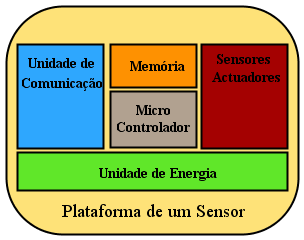
\includegraphics[height=5cm,width=7cm]{SENSOR_NODE.png}
\caption{Modelo de um Sensor de uma RSSF (baseado em
\cite{LIVROARCH_WSN})} \label{fig:sensor_mode}

\end{figure}
\end{center}
Como se pode observar pela figura, da qual se pode generalizar o modelo de uma
plataforma gen�rica de RSSF, os sistemas que est�o presentes s�o os seguintes:
i) Sistema de processamento;ii) Sistema de energia; iii) Sistema de
comunica��o; iv) Sistema sensorial; v) Sistema de mem�ria.
\subsubsection{Arquitectura de \textit{Software} }
Uma das vis�es estruturais da uma RSSF, � a que apresenta pelas camadas de \textit{software} que a
comp�e. Esta vis�o permite ver a plataforma sobre a forma de um conjunto de servi�os que
desempenham tarefas especificas e que lhes permite em cada camada adequar os mecanismos intrinsicos
ao funcionamento, observe-se a figura seguinte que representa esta arquitectura, comparada com o
modelo tradicional das redes 802.2.

\subsubsection{Pilha de Protocolos de uma RSSF }
Uma arquitectura para a a pilha de protocolos em RSSF foi proposta por
\cite{Akyildiz2002}, esta pilha apresenta-se representada por cinco camadas:
\paragraph*{Camada F�sica.}� respons�vel por selec��o de frequ�ncia, detec��o de sinal e modula��o
tendo a minimiza��o do consumo de energia como uma prioridade;
\paragraph*{Camada de Liga��o de Dados.} Das tarefas associadas a estacamada destacam-se as
seguintes: multiplexa��o de dados, acesso ao meio, detec��o de erros/colis�es e detec��o de frames.
Uma RSSF pode ter um protocolo de MAC espec�fico(ex: B-MAC\cite{BMAC}, S-MAC \cite{SMAC}) de modo
agerir o consumo de energia consoante aos protocolos das camadas superiores;
\paragraph*{ Camada de Rede.} sendo a energia um tema transversal a toda a pilha,
esta camada deve endere�ar esta preocupa��o tamb�m, tem como tarefa prim�ria decidir quais os n�s a
escolher para o encaminhamento das mensagens. Um dos sistemas de encaminhamento mais simples � o
baseado na inunda��o (\textit{flooding}), no entanto, apesar da simplicidade n�o tem alguns
problemas como por exemplo: a duplica��o de mensagens e a total ignor�ncia dos recursos da rede,
nomeadamente os energ�ticos. Um dos protocolos que minimiza o impacto da inunda��o � o
SPINS\cite{REF}, negociando e adaptando-se aos recursos existentes;
\paragraph*{Camada de Transporte.} Nas redes convencionais � respons�vel pela  gest�o da congest�o
de tr�fego na rede, gest�o da fiabilidade da comunica��o. Nas RSSF normalmente aparece, muitas
vezes, integrada com  a camada aplica��o
\paragraph*{Camada de Aplica��o.} V�rias s�o as aplica��es desenvolvidas para esta camada,
normalmente, est�o associadas �s capacidades sensoriais das plataformas, que naturalmente est�o
relacionadas com o fim para o qual se instala/desenha a RSSF.

INTRODUZIR AQUI A IMAGEM DA PILHA E DOS SERVI�OS

%Tendo em conta as caracter�sticas das RSSF, toda a pilha � acompanhada transversalmente por
%tr�s planos, que devem ser atendidos por cada uma das camadas, de forma a
%lidarem de forma optima com a energia, mobilidade e recursos partilhados, e
%estes s�o os seguintes: plano de gest�o de tarefas , plano de gest�o
%de energia e plano de gest�o de mobilidade. 
%Esta camada surge com maior relevo quando importa a
%uma infraestrutura de RSSF comunicar com uma rede exterior. No entanto algumas
%das tarefas que podem ser desempenhadas por esta camada acabam por ser
%desempenhadas pela camada de aplica��o, j� que normalmente dizem respeito
%a qualidade de servi�o ou certeza de entrega de  pacotes no destino.
% 
\paragraph{Sistemas de energia}
Como j� tem sido salientado ao longo deste trabalho e pode ser encontrado em
qualquer texto sobre RSSF, a energia � um recurso escasso e como tal deve ser
tomado em conta no desenho de redes de sensores, dependendo tamb�m da aplica��o
ou dos eventos que se pretendem monitorizar bem como a frequ�ncia com que estes
se verificam. Assim, os dispositivos fornecedores de energia podem ser de
diversos tipos, por exemplo: baterias (tipo AA), baterias solares.
Encontra-se nas especifica��es das plataformas mais recentes os valores que
indicam o consumo energ�tico nos diversos estados de opera��o de um
\textit{mote} a titulo de exemplo observe-se a plataforma 
\textit{Mica2}\cite{MICA} da \textit{Crossbows}\cite{CrossbowSite}:
\begin{table*}[ht]
\centering % used for centering table
\begin{tabular}{l r} % centered columns (4 columns)
\hline\hline %inserts double horizontal lines
Descri��o & Valor \\ [0.5ex] % inserts table
%heading
\hline % inserts single horizontal line
Baterias& 2xAA \\ % inserting body of the table
M�nimo $V_{in}$ & 2.7 V \\
Capacidade da bateria& 2000 mAh \\
Regulada &  no \\
\hline %inserts single line
\end{tabular}
\label{table:mica2_caracter} % is used to refer this table in the text
 \caption{Caracter�sticas de energia do \textit{mote} Mica2
(origem:\cite{SNMuseum}))} % title of Table
\end{table*}



\begin{table*}[ht]
\centering % used for centering table
\begin{tabular}{l r} % centered columns (4 columns)
\hline\hline %inserts double horizontal lines
Opera��o & Consumo\\ [0.5ex] % inserts table
%heading
\hline % inserts single horizontal line
CPU \textit{sleep} com \textit{timer} \textit{on} & 0.054 mW \\ % inserting body
CPU activo,\textit{ radio }\textit{off} & 36 mW \\
CPU activo, \textit{radio idle listening }& 66 mW \\
CPU activo, \textit{radio TX/RX }& 117 mW \\
Pot�ncia M�xima (CPU activo, radio TX/RX + flash write) & 165 mW \\ [1ex] %
%[1ex] adds \hline %inserts single line
\end{tabular}
\label{table:mica2_powerops} % is used to refer this table in the text
 \caption{Consumo de Energia \textit{Mica2} - Opera��o Tipica
(origem:\cite{SNMuseum})} % title of Table
\end{table*}
\paragraph{Sistemas de processamento}
O sistema de processamento � um componente essencial num \textit{mote}
\cite{Holger_Karl_protocols_andarchs_wsn}. � respons�vel por recolher
informa��o de todos os sensores do n� process�-la em conformidade, tem ainda de
tratar a informa��o recebida de outros n�s vizinhos. Toda o conjunto de
processamento pode ser realizado nas v�rias arquitecturas representando um
\textit{trade-off} entre desempenho, flexibilidade, performance, custo e
consumo de energia. � semelhan�a do que acontece com os processadores de
computadores convencionais existem microprocessadores gen�ricos que podem ser
aplicados nas mais variadas aplica��es, em especial estes processadores podem
entrar em modos de consumo reduzido (passando para o estado \textit{sleep})
quando n�o est�o a efectuar processamento. Dois dos processadores mais
utilizados nas redes de sensores actuais s�o os da tecnologia Atmel Atmega 128L
\cite{atmel} e da Texas Instruments o controlador TI MSP430 \cite{TIMSP430}

\paragraph{Sistemas de comunica��o}
Este sistema � o respons�vel pela transfer�ncia de dados entre diversos n�s de
uma rede, no caso das RSSF, este sistema � de radio frequ�ncia que permite
dispor de uma rede sem necessidade de infraestrutura de cabos. A
r�dio-frequ�ncia permite ter bom alcance de comunica��o com boas taxas de
transfer�ncia, bem como equilibrar o consumo de energia perante exist�ncia de
erros. Assim para o uso efectivo deste tipo de comunica��o � necess�rio
escolher bem a gama de frequ�ncia de opera��o que tipicamente se situam entre
as gamas 433 Mhz e 2.4Ghz.

Componente ainda fundamental � a existencia de transmissores e receptores
\footnote{No caso da implementa��o em RSSF, as plataformas incorporam num
mesmo componente as duas fun��es, transmiss�o e recep��o, estes s�o denominados
por \textit{transceivers}}nos
n�s. Estes t�m a fun��o de transformar uma cadeia de bits, vindas do
processador, em ondas electromagn�ticas. Os estados pelos quais passam estes
compontes s�o os seguintes e est�o associados essencialmente ao
consumo de energia: a trasmitir\footnote{o trasmissor est� activo e a emitir
dados}, a receber\footnote{O receptor est� activo e a receber dados},
\textit{idle}\footnote{Est� livre para  receber dados, note-se que alguns
componentes de comunica��o est�o activos e outros est�o desligados},
\textit{sleep}\footnote{A maior parte dos componentes de comunica��o est�o
desligados}.
Alguns dos sistemas de r�dio existentes nas redes de sensores s�o os seguintes:
Xemics XE1205 \cite{XEMICS XE1205}, Chipcon 2420 (com chipset para
802.15.4) \cite{CHIPCON2420} 
\paragraph{Sistemas Operativos}
Os sistemas operativos (SO's) para as RSSF s�o menos complexos do que os
restantes SO's comuns para PC's. Esta especificidade deve-se, essencialmente �s
limita��es impostas pelas plataformas de execu��o, os \textit{motes}. Por
exemplo, as aplica��es para RSSF n�o s�o interactivas da� n�o haver
necessidade de implementar interfaces gr�ficas nestes SO's. 
De seguida apresentam-se alguns sistemas operativos com vista a contribuir para
a compreens�o do estado da arte nesta componente das RSSF.
\begin{description}
 \item[TinyOS\cite{tinyos}] Sistema operativo livre e de c�digo aberto,
desenvolvido pela Universidade da California, Berkeley e implementado em nesC
(uma extens�o da linguagem C) muito optimizado para as limita��es de mem�ria
existentes nas RSSF. � composto por diversos componentes, alguns representam
abstrac��es de \textit{hardware} que se ligam por interm�dio de interfaces. O
modelo de execu��o orientado por eventos possibilita uma maior precis�o na
gest�o de energia, ainda assim tem grande flexibilidade no escalonamento dos
eventos gerados pelo ambiente real, que como se sabe s�o de natureza muito
imprevista.
 \item[Contiki\cite{Contiki}] Sistema operativo livre e de c�digo aberto,
implementado em C, e tal como o TinyOS � orientado por eventos. As aplica��es
podem ser carregadas e descarregadas em tempo de execu��o. Os processos deste
SO usam uma \textit{threads} leves, denominadas por protothreads que
proporciona um estilo de programa��o  \textit{threadlike} em cima do
\textit{kernel} orientado a eventos. Uma das inova��es � a possibilidade de com
este SO se ter um modelo \textit{multithreading} por processo bem como um
mecanismo de comunica��o entre processos usando mensagens.
 \item[Nano-RK\cite{nanork}] Sistema operativo desenvolvido na universidade de
Carnegie Mellon, o seu \textit{kernel} � baseado em execu��o em tempo real com 
\textit{multithreading } preemptivo. Assim � possivel ao \textit{kernel}
controlar que processos t�m acesso ao CPU, com a divis�o em frac��es de tempo a
que cada processo acede ao CPU, � rede e aos sensores.
 \end{description}

\paragraph{Exemplos de Plataformas (\textit{motes})}
De forma breve apresentam-se algumas das implementa��es das plataformas usadas
nas RSSF, v�rios s�o os fabricantes e as caracteristicas que as distinguem com
a possibilidade de serem usadas nas mais variadas aplica��es.
A tabela seguinte visa resumir v�rias plataformas:

{
\newcommand{\mc}[3]{\multicolumn{#1}{#2}{#3}}
\begin{table}[ht]
\centering
\begin{scriptsize}
 \begin{tabular}[]{|l||lllll}\cline{1-6}
\mc{6}{|c|}{\textbf{Caracter�sticas de Plataformas de RSSF}}\\\cline{1-6}
& \mc{5}{|c|}{\textbf{\textit{Motes}}}\\\hline\hline
\mc{1}{|c||}{\textbf{Caracter�sticas}} & \mc{1}{|c|}{\textbf{Mica2}} &
\mc{1}{c|}{\textbf{MicaZ}} & \mc{1}{c|}{\textbf{TelosB}} &
\mc{1}{c|}{\textbf{SunSpot}} & \mc{1}{c|}{\textbf{BTNode Rev3}}\\\hline

Micro Controlador & \mc{1}{c|}{Atmel AVR} & \mc{1}{c|}{12} & \mc{1}{c|}{13} &
\mc{1}{c|}{14} & \mc{1}{c|}{15}\\\hline
Energia & \mc{1}{c|}{2xAA / 2000 mAh} & \mc{1}{c|}{22} & \mc{1}{c|}{23} &
\mc{1}{c|}{24} &
\mc{1}{c|}{25}\\\hline
Mem�ria & \mc{1}{c|}{31} & \mc{1}{c|}{32} & \mc{1}{c|}{33} & \mc{1}{c|}{34} &
\mc{1}{c|}{35}\\\hline
Comunica��o & \mc{1}{c|}{Chipcon CC1000/310 MHz } & \mc{1}{c|}{42} &
\mc{1}{c|}{43} & \mc{1}{c|}{44}
& \mc{1}{c|}{45}\\\hline
Sensores/Actuadores & \mc{1}{c|}{51} & \mc{1}{c|}{52} & \mc{1}{c|}{53} &
\mc{1}{c|}{54} & \mc{1}{c|}{55}\\\hline
\end{tabular}
\end{scriptsize}
\caption{Compara��o de Caracter�sticas de Plataformas de RSSF (N�s Sensores)}
\end{table}\label{tab:Caracterisiticas_motes}
}%





\subsection{Modelo de Advers�rio} \label{sect:sec_mod_adversario_serv_seg}
Quando se tratam de quest�es de seguran�a, qualquer se seja o seu dom�nio,
existe uma primeira pergunta que cumpre fazer: ``quais s�o as amea�as/ataques a
que est� sujeito o objecto que se pretende manter seguro?''. Esta pergunta
possibilita, desde logo, encetar uma caminhada que visa a identifica��o de quais
os poss�veis atacantes, que capacidades estes possuem, quais os meios e modos
que estes podem utilizar e em que momento o ataque se pode desencadear. Esta
abordagem, um tanto ou quanto generalista, � suficiente para ilustrar a forma
como se pretende orientar o estudo e com isto apresentar, nas mesmas vertentes,
o modelo de advers�rio que enforma este trabalho.
 \subsubsection{Modelo de Dolev-Yao}\label{sect:subsec_dolev_yao}
Um dos modelos de advers�rio mais conhecidos, quando se trata de
an�lise formal de protocolos seguros, � o modelo de Dolev-Yao \cite{Dolev1983}. 
Assim, neste modelo, � considerado que a rede est� sobre o dom�nio do
advers�rio, que perante este facto pode extrair, reordenar, reenviar, alterar e
apagar as mensagens que circulam entre quaisquer dois principais legitimos. Com
esta assump��o, entende-se portanto, que o advers�rio transporta a mensagem e
com isso adopta um ataque do tipo \textit{man-in-the-middle}\cite{Stall2005},
com
comportamento incorrecto, que o leva a poder alterar o destinat�rio, atribuir
uma falsa origem, analisar o tr�fego ou alterar as mensagens. Este
funcionamento, entenda-se, n�o � comparado � intrus�o mas sim � intercep��o de
mensagens que pode ser mitigado usando mecanismos de criptografia.

As tipologias de ataque, consideradas pelo o modelo de advers�rio de Dolev-Yao
s�o  instanciadas pela norma X800 \cite{ITU-T1991} que pretende
normalizar
uma arquitectura de seguran�a para o modelo OSI, oferecendo uma abordagem
sistem�tica para o desenho de sistemas seguros. Esta norma considera a seguran�a
sobre tr�s aspectos: ataque, mecanismo e servi�o de
seguran�a\cite{Stall2005}. O
primeiro refere-se � forma usada para comprometer um sistema, por exemplo,
alterando ou tendo acesso n�o autorizado autorizado a dados desse sistema. Na
literatura, algumas vezes usam-se os temos ataque e amea�a para denominarem o
mesmo efeito, no entanto recorrendo ao RFC 2828 \cite{RFC2828} podemos
definir amea�a como uma potencial viola��o de seguran�a, ou seja � apenas uma
possibilidade que pode ser usada para desencadear um ataque explorando uma
vulnerabilidade; no caso do ataque, trata-se da explora��o inteligente de uma ou
mais amea�as que resultam na viola��o com sucesso de um sistema que se pretendia
seguro. O segundo aspecto considerado, na norma X.800, s�o os mecanismos de
seguran�a, que se entende como o processo que permite detectar, prevenir ou
recuperar de uma ataque � seguran�a (ex: encripta��o, controlo de acesso,
assinatura digital)\cite{Stall2005}. Por fim, o terceiro aspecto define os
servi�os
que, fazendo uso de um ou mais mecanismos de seguran�a, permitem resistir a
ataques dirigidos a determinada fonte de informa��o, quer seja durante o
processamento ou durante a comunica��o.
 \subsubsection{Modelo de Intrus�o em RSSF}\label{sect:subsec_intrusao}
Considerando o estudo de seguran�a numa RSSF, e dada a sua exposi��o
natural, nomeadamente a f�sica, colocando cada sensor ao alcance de um qualquer
advers�rio, torna relevante a considera��o de novos modelos de ataque.
Considerando que cada rede pode ser constitu�da por milhares de sensores, cada
um deles � um ponto de ataque, na impossibilidade de se proteger ou monitorizar
todos os sensores instalados\cite{Perriga}. Assim
as RSSF v�m-se sujeitas a um modelo de advers�rio que difere das redes com/sem
fios convencionais. Um advers�rio pode estar perto da rede e ter acesso aos
sensores e com isto ``roubar'' um ou parte dos sensores da rede com vista a
explorar os segredos ou material criptogr�fico usados para a comunica��o.
Podemos ent�o tipificar estes ataques como sendo por intrus�o. 
Este tipo de ataques podem ser definidos por ataques desde o n�vel
MAC\cite{Xiao2006} at� ao n�vel de intrus�o f�sica  em que um actor externo,
tendo acesso a um ou m�s sensores leg�timos, descobre os segredos criptogr�ficos
permitindo-lhe replicar\cite{Parno2005} os segredos para sensores maliciosos,
que depois de introduzidos podem agir de forma coordenada comprometendo a rede.
Conseguida a intrus�o, o atacante pode induzir nos sensores leg�timos
comportamentos incorrectos baseados na informa��o falsa introduzida pelos
sensores maliciosos, influenciando o processo de encaminhamento (denominados de
ataques ao encaminhamento).  Note-se, por exemplo, que estes ataques t�m
caracter�sticas que os tornam dif�ceis de identificar quando instalados numa
rede,  uma vez que o car�cter aut�nomo das RSSF, torna dif�cil distinguir um
comportamento errado de uma falha. Um sensor malicioso pode respeitar o
protocolo da rede, no entanto podem actuar de forma incorrecta levando a rede a
criar topologias especificas para o ataque (por exemplo, criando parti��es) ou
fazendo, por exemplo, toda a informa��o passar pelos n�s maliciosos, suprimindo
ou violando a informa��o. No que se refere aos ataques direccionados ao
encaminhamento, por serem parte do objectivo do estudo deste trabalho,
encontram-se definidos na pr�xima sec��o e s�o essencialmente instanciados pela
participa��o colaborativa ou isolada de n�s introduzidos  com o intuito de
afectar o normal funcionamento da rede.
\paragraph{Modelo bizantino: advers�rios bizantinos}
O modelo de ataques por intrus�o tem algumas parecen�as com as denominadas falhas
bizantinas\cite{Falhas_bizantinas}, s�o caracterizadas pela falhas arbitr�rias para as quais um
sistema n�o est�, � partida, preparada para lidar e que se pode traduzir em comportamentos
inesperados do sistema. Transpondo esta realidade para as RSSF, � dificil detectar a introdu��o de
n�s maliciosos, autonomos ou replicados a partir de um de um n� que ficou comprometido. No entanto
alguns autores \cite{PARNO_REPLICATION} t�m-se debru�ado sobre esta problem�tica a fim de dotarem os
algoritmos de mecanismos que permitam detectar a replica��o de n�s maliciosos numa RSSF.
Para se lidar com os ataques com comportamentos bizantinos, implementam-se mecanismos
probabilisticos que ainda que n�o possam mitigar o ataque por completo aumentam a resili�ncia e
acabam por transformar um ataque num mal menor, definindo at� onde pode ser comprometida a rede, ou
seja qual o n�mero de n�s que poder�o estar comprometidos mas que apesar disso a rede continua a
garantir a fiabilidade necess�ria para a opera��o.

 \subparagraph{Sum�rio}
    Mediante as vulnerabilidades de uma RSSF, � necess�rio estabelecer um modelo
de advers�rio com vista a poder mapear as capacidades e tipologias de ataques
deste em mecanismos de seguran�a com o prop�sito de lhes poder resistir ou
mitiga-los. O modelo de Dolev-Yao � o modelo de facto quando se trata da an�lise
de amea�as a redes , em que o meio de comunica��o est� sobre controlo do
advers�rio. No entanto, tratando-se de RSSF, este modelo per si n�o se vislumbra
suficiente para abarcar todas as problem�ticas de seguran�a a que este tipo de
redes est� sujeita. Surge assim a necessidade de, face � inseguran�a que cada n�
da rede representa, estender este modelo acrescentando-lhe um modelo de
intrus�o.
    Perante a exposi��o das RSSF, os ataques que se podem desencadear podem ser
diferentes dos observados nas redes convencionais sendo assim necess�rio
considerar outras tipologias de ataques. Assim, podemos classificar os ataques
como activos e passivos \cite{Stallings2005} e os atacantes como internos e
externos\cite{Karlof2003}.
Nestes ultimos ainda se pode classificar quanto aos recursos usados como
\textit{sensor-class} ou \textit{laptop-class}\cite{Karlof2003}. Os ataques que
se consideram para o estudo e
relacionados com as RSSF s�o: falsa informa��o de encaminhamento,
\textit{blackhole},\textit{sinkhole}, \textit{wormhole} e  \textit{sybil
attack}\cite{Douceur2002}.

 
%REVISTO
\subsection{Arquitectura de Servi�os de Seguran�a em
RSSF} \label{sect:subsec_arq_security_wsn}
Num sistema seguro, � necess�rio que a seguran�a esteja integrada em cada um dos seus componentes, 
n�o se confinando a um componente isolado do sistema\cite{sec_in_wsn_perrig}.
Assim, nesta sec��o apresenta-se, introdutoriamente, alguns requisitos de seguran�a de uma RSSF e 
alguns servi�os de seguran�a, que foram implementados com o objectivo de
representarem um ponto de partida para a garantia de propriedades de seguran�a, a quando do desenho
de RSSF seguras.
\subsubsection{Requisitos de seguran�a de uma RSSF}
Os requisitos de seguran�a de uma RSSF podem variar consoante as especificidades da aplica��o que a
rede visa suportar. No entanto, apresentam-se, de forma gen�rica, os principais requisitos de
seguran�a de uma RSSF\cite{sec_in_wsn_perrig}:
\begin{description}\descvspace
 \item[Autentica��o]
Devido ao meio de comunica��o ser partilhado, � necess�rio recorrer � autentica��o para garantir a
detec��o de mensagens alteradas ou injectadas no sistema por participantes n�o
 autorizados\cite{sec_in_wsn_perrig}. Note-se que a implementa��o de criptografia assim�trica
contribui para a garantia desta propriedade, mas ainda existe muito esfor�o a desenvolver neste
campo dadas as limita��es das RSSF e as exig�ncias computacionais e energ�ticas destes
mecanismos.
 \item[Confidencialidade]
Sendo a RSSF uma infraestrutura baseada fundamentalmente na dissemina��o de dados recolhidos a
partir de sensores que se encontram distribuidos em ambiente n�o controlado e, normalmente, de
f�cil acesso,  � necess�rio garantir a confidencialidade dos dados que circulam na rede.
Assim, o uso de mecanismos de criptografia � o mais indicado para este tipo de protec��o.Desta
forma, � necess�ria a utiliza��o de algoritmos de encripta��o fi�veis (ex:
AES\footnote{\textit{Advenced Encryption System algorithm}}\cite{Stallings2005},
ECC\cite{Stallings2005}) para garantir
um determinado n�vel de seguran�a, para isso existe a necessidade de partilhar chaves de sess�o por
todos os \textit{end-points} e como tal deve-se recorrer a esquemas de distribui��o de
chaves\cite{eschenauer2002}.
 \item[Disponibilidade]
Entende-se por disponibilidade de uma rede, a garantia de que esta funciona efectivamente
durante o seu tempo de opera��o. Os ataques por nega��o de servi�o (Denial of Service -
DoS)\cite{Hu2005} s�o os mais frequentes para diminuir a disponibilidade de uma rede. Ent�o, para
al�m de mecanismos que evitem a nega��o de servi�o, � necess�rio garantir que a degrada��o da
rede (ex: na presen�a de um ataque ) seja controlada e que v� sendo proporcional ao n�mero de n�s
comprometidos.
 \item[Integridade]
A integridade garante que os dados recebidos por um n� n�o foram alterados, por um
advers�rio, durante a transmiss�o. Em alguns casos esta propriedade � garantida juntamente com a
autentica��o, usando mecanismos que permitam garantir ambos numa s� opera��o. Por exemplo, o uso de
CMAC's\cite{Stallings2005} � vulgar uma vez que permite autenticar (uso de critografia sim�trica)
a mensagem e para garantir a integridade da mensagem.\cite{SPINS}.
\item[Frescura]
A frescura de uma mensagem implica que estes sejam recentes, garantindo que esta n�o � antiga
e n�o foi reenviada por um qualquer advers�rio. \cite{SPINS,Luk2007d} Podem-se considerar dois tipos
de frescura: frescura fraca (garantindo ordem parcial e sem informa��o do desvio de tempo, usada
para as medi��es dos sensores) e frescura forte (garante ordem total em cada
comunica��o permitindo estimar o atraso, usada para a sincroniza��o de tempo).
 \end{description}
\subsubsection{Servi�os de Seguran�a}
Alguns servi�os de seguran�a t�m vindo a ser desenvolvidos para as RSSF com vista a garantir a
seguran�a ao n�vel da comunica��o (ex: criptografia, assinaturas, \textit{digests}). Estes servi�os
permitem que o arquitecto de sistemas se centre em outras problem�ticas relacionadas com o
comportamento dos protocolos face outros ataques. Apresentam-se de seguida alguns servi�os mais
comuns:
\begin{description}\addtolength{\itemsep}{-0.5\baselineskip}
\item[TinySec\cite{Karlof2004}]
TinySec � uma arquitectura de seguran�a para protec��o ao n�vel de liga��o de
dados em RSSF. O objectivo principal, para o qual foi desenhado, � providenciar
um n�vel adequado de seguran�a com o m�nimo consumo de recursos. Os servi�os de
seguran�a  disponibilizados s�o: autentica��o de dados (com a utiliza��o de
\textit{Message Authentication Codes}(MAC)\cite{Stallings2005}, no caso CBC-MAC\footnote{Cipher
Block Chaining - Message Authentication Code (CBC-MAC))}) e confidencialidade (CBC-MAC).
N�o implementa nenhum mecanismo que garanta a frescura das mensagens, tornando-o vulner�vel a
ataques de \textit{replaying}).
\item[MiniSec\cite{Luk2007d}]
Minisec � uma camada de rede concebida para possuir baixo consumo de energia, melhor que o TinySec,
e alta seguran�a. Uma das caracteristicas principais, que a tornam mais eficiente, � o uso do modo
\textit{offset codebook} (OCB)\cite{Stallings2005}  para encripta��o de blocos. O que permite numa
�nica passagem autenticar e encriptar os dados, sem com isso aumentar o tamanho da mensagem em
claro, contribuindo para um menor consumo de energia. Esta arquitectura tem dois modos de opera��o:
uma baseado paracomunica��o \textit{unicast} (MINISEC-U) e outro para \textit{broadcast}
(MINISEC-B). Sendo que a segunda n�o necessita de manter o estado (sincroniza��o de contadores) por
cada emissor por forma a proteger o reenvio escalando para grandes redes.
\item[SPINS\cite{SPINS}]
Conjunto de protocolos de seguran�a, constitu�do por dois componentes
principais SNEP\footnote{Secure Network Encryption Protocol} \cite{SPINS} e
${\mu}$TESLA \cite{SPINS,Luk2006}. O primeiro, fornece servi�os de autentica��o e
confidencialidade entre dois pontos de comunica��o, encriptando as mensagens (com
o modo CTR\footnote{\textit{Counter Mode}}) e protegendo-as com um MAC (autentica��o com CBC-MAC). O
SNEP gera diferentes chaves, de encripta��o, que derivam de uma chave mestra partilhada entre os
dois n�s, com umcontador de mensagens para garantir a frescura. O segundo componente,o
${\mu}$TESLA\cite{SPINS,Luk2006}, � um servi�o de autentica��o de \textit{broadcast}, que evita a
utiliza��o de mecanismos, mais exigentes, de criptografia assim�trica, recorrendo a critografia
sim�trica, autenticando as mensagens com um MAC, 
\item[Norma IEEE802.15.4\cite{ietf_802154}]
Esta norma define a especifica��o da camada f�sica e de controlo de acesso ao meio das redes
pessoais de baixa pot�ncia (\textit{LRPAN}\footnote{Low Rate Personal Area Networks}). Foca-se
essencialmente na comunica��o entre dispositivos relativamente pr�ximos, sem a
necessidade de uma infrastrutura de suporte, explorando o m�nimo de consumo de energia. � a norma
que j� se encontra implementada em algumas plataformas das RSSF. (ex: Micaz\cite{micaz}).
Esta norma, especifica alguns servi�os de seguran�a\cite{zigbee_802154}, representam uma primeira
linha de protec��o contra ataques � infraestrutura. Estes mecanimos s�o os seguintes: i) Cada
dispositivo mant�m uma lista de controlo de acessos (ACL) dos dispositivos confi�veis
filtrando comunica��es n�o autorizadas; ii) Encripta��o de dados, partilha de uma chave
criptogr�fica entre os intervenientes na comunica��o; iii) Servi�o de integridade de cada
\textit{frame}, adicionando a cada frame uma \textit{Message Integrity Code}
(MIC)\cite{Stallings2005}; iv) Garantia de frescura de mensagens (\textit{Sequential Freshness}),
utilizando contadores de frames e de chaves.
\item[ZigBee\cite{zigbee_802154,zigbee}]
Com a norma 802.15.4 orientada para as duas camadas mais baixas da pilha de
protocolos das RSSF (f�sica e MAC), a norma ZigBee define as especifica��es para
a camada de rede e aplica��o. J� incorpora alguns servi�os de seguran�a, nomeadamente: i) Frescura,
mantendo contadores associados a cada chave de sess�o, que s�o reiniciados em cada mudan�a de chave;
ii) Integridade, com op��es de integridade de mensagens que v�o desde os 0 aos 128 bits de
verifica��o; ii) Autentica��o, ao n�vel de rede e ao n�vel de liga��o de dados;
iv) Confidencialidade, com o algoritmo AES\cite{Stallings2005} com 128 bits.
Esta arquitectura utiliza um \textit{trusted center} para gest�o da seguran�a na rede,
implementando um coordenador de rede ZigBee. Este, acreditado por todos os n�s da rede, pode
desempenhar tr�s fun��es: i) Autentica��o de n�s que pretendem participar na rede; ii) Manuten��o e
distribui��o de chaves; iii) Providenciar seguran�a ponto-a-ponto entre n�s da rede.
\end{description}